\chapter{Widgets}

 
\section{BleConfigWidget}

The BleConfigWidget is a specialized widget in your dashboard application designed to interact with the tag device, retrieve configuration data from it, and update the configuration remotely. 

In order to view the current configuration and change it, go through the following steps. 
%
\begin{enumerate}
	\item Add the BleConfigWidget widget to your dashboard. Drag and resize it if needed. 
	\item On the Tag device hit the user button 1 and look for a change in the user LEDs. When the config mode is entered the should blink in a repetetive pattern. 
	\item Hit the "Refresh" button and wait for a few seconds for your device to scan the vicinity for Bluetooth devices. 
	\item Select the "ESP32" device from the device list right to the Refresh button. 
	\item Hit the "Connect" button. After a short time the saved coordinates for each anchor device start to appear in the corresponding text fields. 
	\item To change the coordinates, define them in your setup physical by measuring thei position in relation to the origin (0,0,0). 
	\item Simpy change the already displayed coordinates. once the system noticed a change in a certain value the cell will change its color to red. 
	\item Once you are finished reconfigurating you need to hit the "Upload" button below the displayed coordinates to transfer the new values to the tag device. 
	\item To initiate the saving process you hit the "Save Config". The Tag device will automatically update the values by writing them into its EEPROM and reboot. 
\end{enumerate}
%
\newpage
%
\begin{figure}[!hbt]
	\centering
	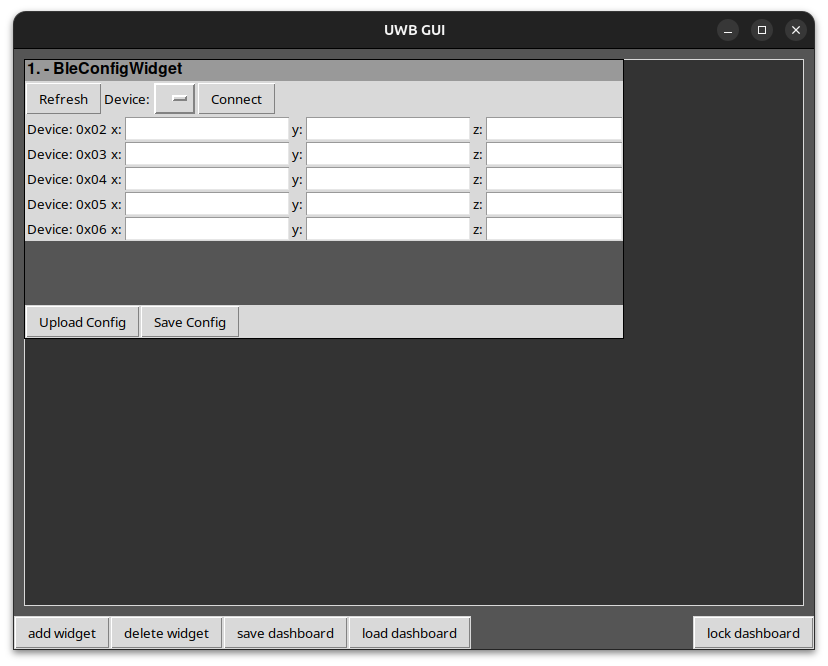
\includegraphics[width=0.42\textwidth]{pictures/cofig_device_idle.png}
	\caption{Empty configuration widget before connecting.}
	\label{fig:cofig_device_idle}
\end{figure}

\begin{figure}[!hbt]
	\centering
	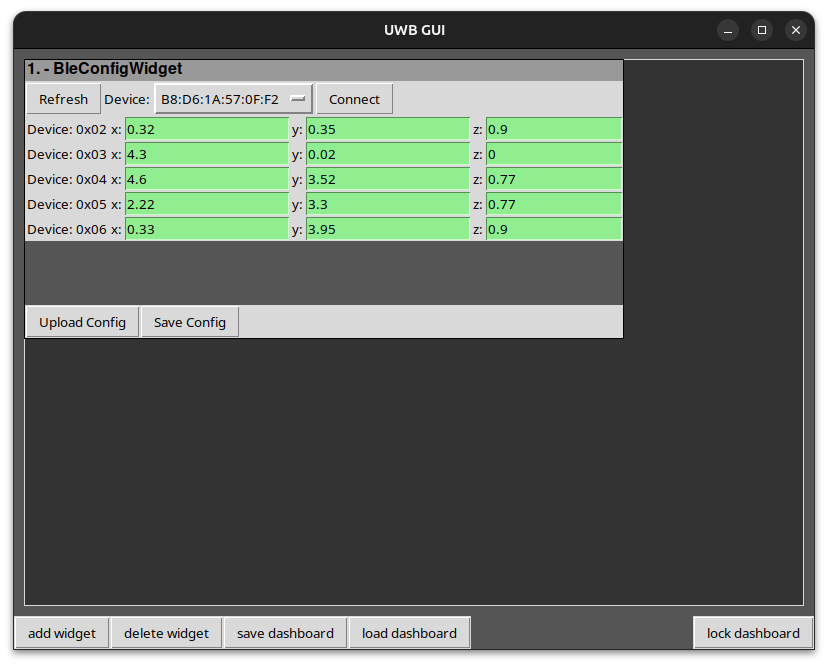
\includegraphics[width=0.42\textwidth]{pictures/config_device_connected.png}
	\caption{Configuration widget is displaying the currently saced coordinates after connecting successfully.}
	\label{fig:config_device_connected}
\end{figure}

\begin{figure}[!hbt]
	\centering
	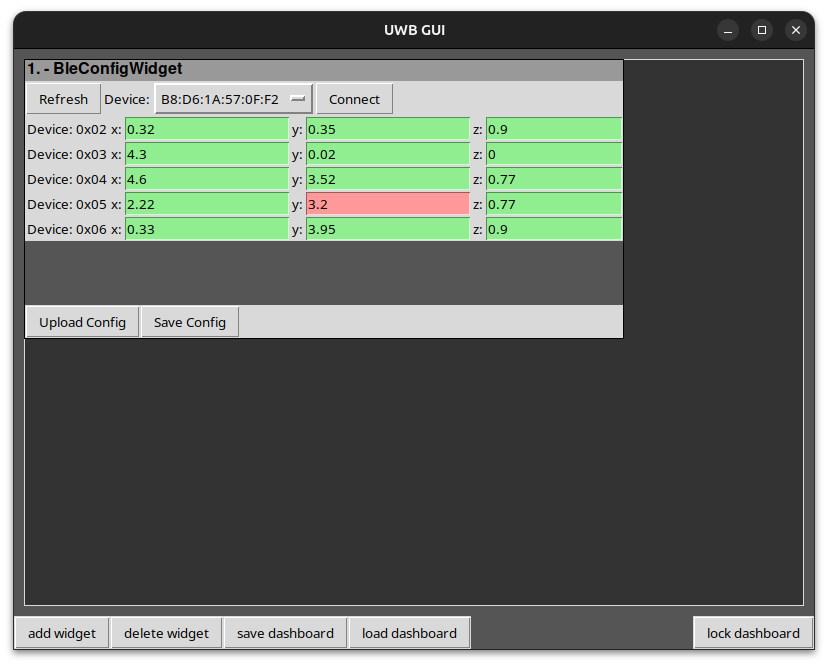
\includegraphics[width=0.42\textwidth]{pictures/config_coordinate_changed.png}
	\caption{Configuration widget is displaying the changed coordinate in red. }
	\label{fig:config_coordinate_changed}
\end{figure}

\newpage

\section{BlePlotPositionWidget}

The BlePlotPositionWidget lets you display the current position of the tag in the choosen coordinate system. 
In order to use it properly use it go through the following steps. 

\begin{enumerate}
	\item Add the BleConfigWidget widget to your dashboard. Drag and resize it if needed. 
	\item Make sure that all anchor devices 0x02 to 0x06 are up and running properly. Otherwise the estimated position may vary a lot. 
	\item Make sure the tag device is running and in uwb mode. That state is given if the LED 1 is consistently on and the green RX and TX LEDs next to the DWM3000 chip are blinking repetitively, if activated. 
	\item Hit the "Refresh" button and wait for a few seconds for your device to scan the vicinity for Bluetooth devices. 
	\item Select the "ESP32" device from the device list right to the Refresh button. 
	\item Hit the "Connect" button. After a short time the saved coordinates for each anchor device. 
	\item Now in the given plot of the widget a dot with the current estimated position is added. 
\end{enumerate}

\begin{figure}[!hbt]
	\centering
	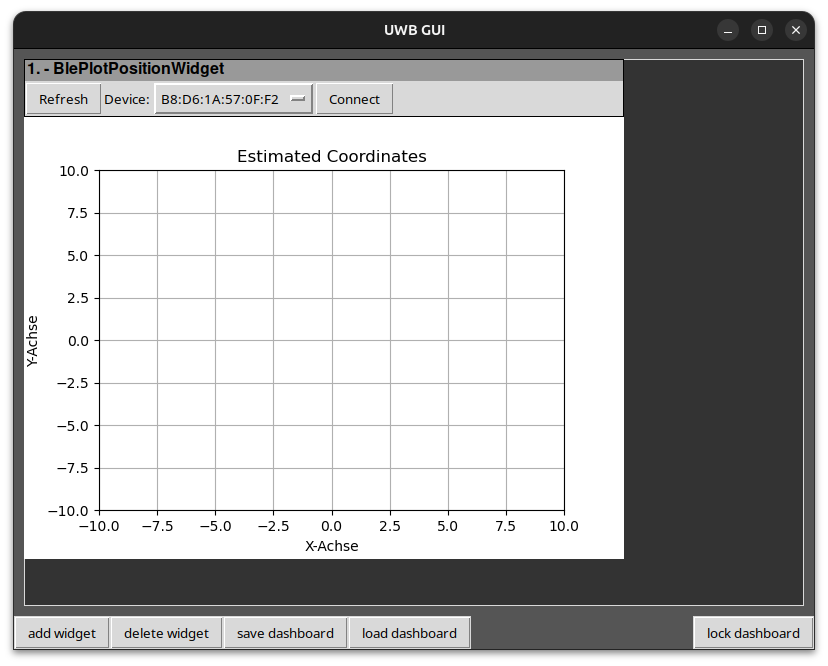
\includegraphics[width=0.6\textwidth]{pictures/coordinate_plot.png}
	\caption{Plot Position Widget with no position currently displayed.}
	\label{fig:coordinate_plot}
\end{figure}
